Svi zadaci ostvareni su u okviru učenja pretraživanja koji je implementiran u
sustavu za strojno učenje zvanom Vowpal Wabbit. U dodacima
\ref{appendix:postagging}, \ref{appendix:msdattr}, \ref{appendix:msdlayered}
prikazana je jednostavnost implementacije za zadatke označavanja vrste riječi.
Korišten je programski jezik \textsc{C++}. Moguće je sve zadatke izvesti u
jeziku \textsc{Python}, ali ušteda u čitljivosti smanjuje vremensku
učinkovitost. Uzevši u obzir da je okvir učenja pretraživanja poprilično
modularan tijekom implementacije greške su uglavnom bile prisutne u krivoj
obradi podataka i odabiru hiperparametara. \textit{Hashing trick} dozvoljava
običan tekstualni format za svaku značajku stoga je ulazna datoteka vrlo
jednostavna (dodatak \ref{appendix:data}).

Obrada podataka i njihova pretvorba u prikladan oblik vektora značajki za
potrebe sustava Vowpal Wabbit izvršena je koristeći alate ljuske \engl{shell}.
Neki od  bitnijih su
\begin{inlinelist}
  \item \textsc{sed},
  \item \textsc{cut},
  \item \textsc{diff},
  \item \textsc{shuf} i
  \item \textsc{awk}.
\end{inlinelist}
\textsc{Awk} je ubrzao kreiranje značajki i zbog prikladnog standardnog
ponašanja sve napisane skripte rade za označene i neoznačene podatke.
\textsc{Shuf} dopušta vrlo jednostavno miješanje rečenica i stvaranje drugačijih
skupova za učenje, testiranje i razvoj. \textsc{Diff} je korišten za računanje
metrike točnosti. Zbog stupčastog formata podatkovnih skupova \textsc{Cut} i
\textsc{sed} korišteni su za jednostavnu selekciju stupaca, laku izmjenu
sadržaja i filtriranje komentara. Svi navedeni alati trebali bi biti prisutni na
standardnoj distribuciji \textsc{Ubuntu}. Čitatelja se upućuje na dokumentaciju
izvornog koda koja je priložena zajedno s elektronskom verzijom rada.

U okviru ovog rada, u sustavu Vowpal Wabbit, implementirana su rješenja za
sljedeće probleme obrađene u prijašnjim poglavljima:
\begin{inlinelist}
  \item označavanje vrste riječi,
  \item označavanje vrste riječi s više prolaza,
  \item označavanje vrste riječi koristeći morfosintaktičke deskriptore
  \engla{morphosyntactic descriptor}{msd} po atributima,
  \item označavanje vrste riječi koristeći morfosintaktičke deskriptore po
  razinama,
  \item ovisnosno parsanje,
  \item združeno ovisnosno parsanje i označavanje vrste riječi i
  \item združeno ovisnosno parsanje i označavanje vrste riječi koristeći
  morfosintaktičke deskriptore.
\end{inlinelist}
Rezultati za svaki pristup prikazani su u nastavku.

\citet{daume14lts} opisuju efikasnu implementaciju okvira učenja pretraživanja.
Na slici \ref{fig:ltsperf} prikazana je vremenska učinkovitost sustava na
zadatku označavanja vrste riječi i imenovanim entitetima -- broj označenih
tokena po sekundi. Učinkovitost je prisutna i kod ostvarenih rješenja za
probleme obrađene u okviru ovog rada.

\begin{figure}
  \centering
  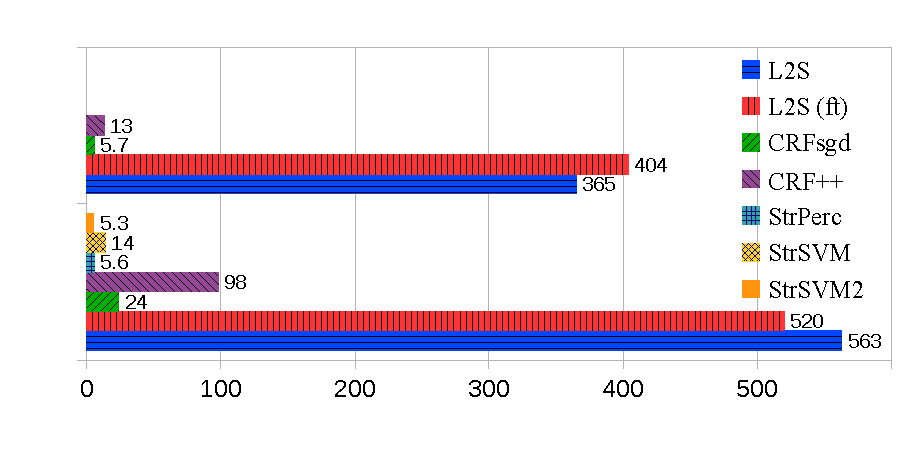
\includegraphics[scale=0.9]{tokenposec.pdf}
  \caption[Usporedba brzine označavanja metoda strukturnog
  predviđanja.]{Usporedba brzine označavanja metoda strukturnog predviđanja.
  Prikazani brojevi su u tisućama po sekundi. Slika se u izvornom obliku nalazi
  u \citep{ltsicmltutorial}.}
  \label{fig:ltsperf}
\end{figure}
